\begin{figure}[h]
\centering
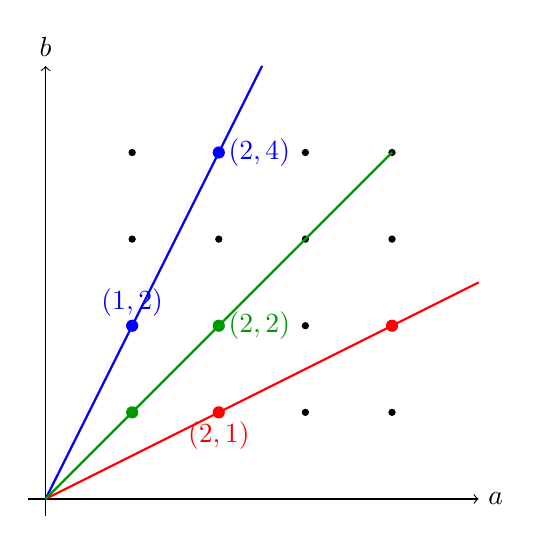
\begin{tikzpicture}[scale=1.1]

% axes
\draw[->] (-0.2,0) -- (5,0) node[right] {$a$};
\draw[->] (0,-0.2) -- (0,5) node[above] {$b$};

% lattice points
\foreach \x in {1,2,3,4}
  \foreach \y in {1,2,3,4}
    \fill (\x,\y) circle (1.2pt);

% rational lines
\draw[blue, thick] (0,0) -- (2.5,5);
\draw[red, thick] (0,0) -- (5,2.5);
\draw[green!60!black, thick] (0,0) -- (4,4);

% example points
\fill[blue] (1,2) circle (2pt);
\fill[blue] (2,4) circle (2pt);

\fill[red] (2,1) circle (2pt);
\fill[red] (4,2) circle (2pt);

\fill[green!60!black] (1,1) circle (2pt);
\fill[green!60!black] (2,2) circle (2pt);

% labels
\node[blue,right] at (2,4) {$(2,4)$};
\node[blue,above] at (1,2) {$(1,2)$};

\node[red,below] at (2,1) {$(2,1)$};

\node[green!60!black,right] at (2,2) {$(2,2)$};

\end{tikzpicture}

\caption{Integer pairs representing the same rational number lie on the same line through the origin.}
\end{figure}

\FloatBarrier